% **************************************************
% Document Class Definition
% **************************************************
\documentclass[%
    paper=A4,               % paper size --> A4 is default in Germany
    twoside=true,           % onesite or twoside printing
    openright,              % doublepage cleaning ends up right side
    parskip=half,           % spacing value / method for paragraphs
    chapterprefix=true,     % prefix for chapter marks
    11pt,                   % font size
    headings=normal,        % size of headings
    bibliography=totoc,     % include bib in toc
    listof=totoc,           % include listof entries in toc
    titlepage=on,           % own page for each title page
    captions=tableabove,    % display table captions above the float env
    chapterprefix=false,    % do not display a prefix for chapters
    appendixprefix=false,    % but display a prefix for appendix chapter
    draft=false,            % value for draft version
]{scrreprt}%


% **************************************************
% Setup YOUR thesis document in this file !
% **************************************************
% !TEX root = my-thesis.tex


% **************************************************
% Files' Character Encoding
% **************************************************
\PassOptionsToPackage{utf8}{inputenc}
\usepackage{inputenc}


% **************************************************
% Information and Commands for Reuse
% **************************************************
\newcommand{\thesisTitle}{TITLE goes here}
\newcommand{\thesisName}{Nima Karimi}
\newcommand{\thesisSubject}{Documentation}
\newcommand{\thesisDate}{July 04, 2023}
\newcommand{\thesisVersion}{My First Draft}

\newcommand{\thesisFirstReviewer}{Jane Doe}
\newcommand{\thesisFirstReviewerUniversity}{\protect{Clean Thesis Style University}}
\newcommand{\thesisFirstReviewerDepartment}{Department of Clean Thesis Style}

\newcommand{\thesisSecondReviewer}{John Doe}
\newcommand{\thesisSecondReviewerUniversity}{\protect{Clean Thesis Style University}}
\newcommand{\thesisSecondReviewerDepartment}{Department of Clean Thesis Style}

\newcommand{\thesisFirstSupervisor}{Jane Doe}
\newcommand{\thesisSecondSupervisor}{John Smith}

\newcommand{\thesisUniversity}{\protect{University of Padova}}
\newcommand{\thesisUniversityDepartment}{Department of Management Engineering}
\newcommand{\thesisUniversityInstitute}{Institute for Clean Thesis Dev}
\newcommand{\thesisUniversityGroup}{Dipartimento di Tecnica e Gestione dei sistemi industriali}
\newcommand{\thesisUniversityCity}{Padova}
\newcommand{\thesisUniversityStreetAddress}{Street address}
\newcommand{\thesisUniversityPostalCode}{Postal Code}


% **************************************************
% Debug LaTeX Information
% **************************************************
%\listfiles


% **************************************************
% Load and Configure Packages
% **************************************************
\usepackage[english]{babel} % babel system, adjust the language of the content
\PassOptionsToPackage{% setup clean thesis style
    figuresep=colon,%
    hangfigurecaption=false,%
    hangsection=true,%
    hangsubsection=true,%
    sansserif=false,%
    configurelistings=true,%
    colorize=full,%
    colortheme=bluemagenta,%
    configurebiblatex=true,%
    bibsys=biber,%
    bibfile=bib-refs,%
    bibstyle=numeric,%
    bibsorting=nty,%
}{cleanthesis}
\usepackage{cleanthesis}

\hypersetup{% setup the hyperref-package options
    pdftitle={\thesisTitle},    %   - title (PDF meta)
    pdfsubject={\thesisSubject},%   - subject (PDF meta)
    pdfauthor={\thesisName},    %   - author (PDF meta)
    plainpages=false,           %   -
    colorlinks=true,           %   - colorize links?
    linkcolor=BlueViolet,
    urlcolor=blue,
    citecolor=blue,
    % allcolors=blue,
    pdfborder={0 0 0},          %   -
    breaklinks=true,            %   - allow line break inside links
    bookmarksnumbered=true,     %
    bookmarksopen=true          %
}

% **************************************************
% Other Packages
% **************************************************
\usepackage{scrhack}


% **************************************************
% Document CONTENT
% **************************************************
\begin{document}

% uncomment the following command to fill up pages with
% whitespace instead of aligning the first and last lines
% of a page (see \raggedbottom vs. \flushbottom)
%\raggedbottom

% --------------------------
% rename document parts
% --------------------------

% > set short label names for floating environments figure and table
%\renewcaptionname{ngerman}{\figurename}{Abb.}
%\renewcaptionname{ngerman}{\tablename}{Tab.}
\renewcaptionname{english}{\figurename}{Fig.}
\renewcaptionname{english}{\tablename}{Tab.}

% > rename the title of the LOL, i.e. list of listings (default is "Listings")
\renewcommand*{\lstlistlistingname}{List of Listings}

% --------------------------
% Front matter
% --------------------------
\pagenumbering{roman}			% roman page numbing (invisible for empty page style)
\pagestyle{empty}				% no header or footers
% !TEX root = ../my-thesis.tex
%
% ------------------------------------  --> cover title page
\begin{titlepage}
	\pdfbookmark[0]{Cover}{Cover}
	\flushright
	\hfill
	\vfill
	\vbox to0pt{\vbox to\textheight{\vfill 
\includegraphics[width=11.5cm]{resources/unipd-light} \vfill}\vss}
	{\LARGE\thesisTitle \par}
	\rule[5pt]{\textwidth}{.4pt} \par
	{\Large\thesisName}
	\vfill
	\textit{\large\thesisDate} \\
	Version: \thesisVersion
\end{titlepage}


% ------------------------------------  --> main title page
\begin{titlepage}
	\pdfbookmark[0]{Titlepage}{Titlepage}
	\tgherosfont
	\centering

	{\Large \thesisUniversity} \\[4mm]
	
\includegraphics[width=6cm]{gfx/Clean-Thesis-Logo} \\[2mm]
	\textsf{\thesisUniversityDepartment} \\
	\textsf{\thesisUniversityInstitute} \\
	\textsf{\thesisUniversityGroup} \\

	\vfill
	{\large \thesisSubject} \\[5mm]
	{\LARGE \color{ctcolortitle}\textbf{\thesisTitle} \\[10mm]}
	{\Large \thesisName} \\

	\vfill
	\begin{minipage}[t]{.27\textwidth}
		\raggedleft
		\textit{1. Reviewer}
	\end{minipage}
	\hspace*{15pt}
	\begin{minipage}[t]{.65\textwidth}
		{\Large \thesisFirstReviewer} \\
	  	{\small \thesisFirstReviewerDepartment} \\[-1mm]
		{\small \thesisFirstReviewerUniversity}
	\end{minipage} \\[5mm]
	\begin{minipage}[t]{.27\textwidth}
		\raggedleft
		\textit{2. Reviewer}
	\end{minipage}
	\hspace*{15pt}
	\begin{minipage}[t]{.65\textwidth}
		{\Large \thesisSecondReviewer} \\
	  	{\small \thesisSecondReviewerDepartment} \\[-1mm]
		{\small \thesisSecondReviewerUniversity}
	\end{minipage} \\[10mm]
	\begin{minipage}[t]{.27\textwidth}
		\raggedleft
		\textit{Supervisors}
	\end{minipage}
	\hspace*{15pt}
	\begin{minipage}[t]{.65\textwidth}
		\thesisFirstSupervisor\ and \thesisSecondSupervisor
	\end{minipage} \\[10mm]

	\thesisDate \\

\end{titlepage}


% ------------------------------------  --> lower title back for single page layout
\hfill
\vfill
{
	\small
	\textbf{\thesisName} \\
	\textit{\thesisTitle} \\
	\thesisSubject, \thesisDate \\
	Reviewers: \thesisFirstReviewer\ and \thesisSecondReviewer \\
	Supervisors: \thesisFirstSupervisor\ and \thesisSecondSupervisor \\[1.5em]
	\textbf{\thesisUniversity} \\
	\textit{\thesisUniversityGroup} \\
	\thesisUniversityInstitute \\
	\thesisUniversityDepartment \\
	\thesisUniversityStreetAddress \\
	\thesisUniversityPostalCode\ and \thesisUniversityCity
}
		% INCLUDE: all titlepages
\cleardoublepage

\pagestyle{plain}				% display just page numbers
% !TEX root = ../my-thesis.tex
%
\pdfbookmark[0]{Abstract}{Abstract}
\addchap*{Abstract}
\label{sec:abstract}

\blindtext

\vspace*{20mm}

{\usekomafont{chapter}Abstract (different language)}
\label{sec:abstract-diff}

\blindtext
		% INCLUDE: the abstracts (english and german)
\cleardoublepage
%
% !TEX root = ../my-thesis.tex
%
\pdfbookmark[0]{Acknowledgement}{Acknowledgement}
\addchap*{Acknowledgement}
\label{sec:acknowledgement}

\Blindtext[2][2]
 % INCLUDE: acknowledgement
\cleardoublepage
%
\currentpdfbookmark{\contentsname}{toc}
\setcounter{tocdepth}{2}		% define depth of toc
\tableofcontents				% display table of contents
\cleardoublepage

% --------------------------
% Body matter
% --------------------------
\pagenumbering{arabic}			% arabic page numbering
\setcounter{page}{1}			% set page counter
\pagestyle{scrheadings}			% header and footer style

%% Uncomment the following lines using the \part command
%% to add part sections
%\part{Example Part}
% !TEX root = ../my-thesis.tex
%
\chapter{Introduction}
\label{sec:intro}
With the rapid expansion of cities and the escalating worries regarding the sustainable use of our natural resources, the quest for achieving transportation systems that are not only efficient but also eco-friendly has garnered significant attention and become an urgent global challenge. 
Sustainable mobility, often referred to as sustainable transportation, aims to develop and implement strategies that promote the efficient movement of people and goods while minimizing negative environmental and social impacts. 
% Machine learning, a field of artificial intelligence, has emerged as a promising approach to addressing the complexities inherent in sustainable mobility by leveraging data-driven insights and advanced computational algorithms.

Furthermore, machine learning, a field of artificial intelligence, involves the development and application of computational models that can automatically learn and improve from data without explicit programming. By analyzing large and diverse datasets, machine learning algorithms can identify patterns, make predictions, and gain valuable insights that aid decision-making processes. In the context of sustainable mobility, machine learning can provide innovative solutions to optimize transportation systems, improve accessibility, and minimize environmental impact.

Optimizing transportation systems through machine learning involves the application of data analytics to enhance operational efficiency, reduce congestion, and improve the overall performance of transportation networks. By processing large volumes of data collected from sources such as traffic sensors, GPS devices, and social media platforms, machine learning algorithms can generate real-time traffic predictions, optimize routing, and dynamically adapt transportation services. These advancements lead to improved travel experiences, reduced travel times, and more efficient allocation of resources.

Accessibility is a key aspect of sustainable mobility, aiming to ensure that transportation services are available and equitable for all individuals, regardless of their physical abilities, income levels, or geographic location. Machine learning algorithms can help address accessibility challenges by analyzing data on travel demand, demographics, and infrastructure characteristics. This enables the identification of underserved areas, optimization of transit routes, and the design of transportation services that cater to the needs of diverse populations.

Environmental sustainability is another critical dimension of sustainable mobility. Transportation accounts for a significant portion of global greenhouse gas emissions and is a major contributor to air pollution. Machine learning can play a crucial role in minimizing the environmental impact of transportation by developing predictive models that estimate emissions, optimize energy consumption, and facilitate the integration of clean and renewable energy sources. Additionally, machine learning techniques can aid in the design of eco-routing algorithms, which suggest the most environmentally friendly travel routes based on real-time data.

In summary, the combination of machine learning and sustainable mobility presents a promising framework to address the complex challenges faced by transportation systems. By harnessing the power of machine learning algorithms, transportation stakeholders can optimize operations, improve accessibility, and mitigate environmental impact. As the demand for sustainable and efficient mobility solutions continues to grow, machine learning can provide valuable insights and tools to shape the future of transportation, leading to more sustainable, accessible, and environmentally friendly mobility systems.




\section{Motivation and Problem Statement}
\label{sec:intro:motivation}

\Blindtext[3][1] \cite{Jurgens:2000,Jurgens:1995,Miede:2011,Kohm:2011,Apple:keynote:2010,Apple:numbers:2010,Apple:pages:2010}

\section{Results}
\label{sec:intro:results}

\Blindtext[1][2]

\subsection{Some References}
\label{sec:intro:results:refs}

\cite{WEB:GNU:GPL:2010,WEB:Miede:2011}
\Blindtext[1][1]

\subsubsection{Methodology}
\label{sec:intro:results:refs:method}

\Blindtext[1][2]

\paragraph{Strategy 1}
\Blindtext[1][1]

\begin{lstlisting}[language=Python, caption={This simple helloworld.py file prints Hello World.}\label{lst:pyhelloworld}]
#!/usr/bin/env python
print "Hello World"
\end{lstlisting}

\paragraph{Strategy 2}
\Blindtext[1][1]

\begin{lstlisting}[language=Python, caption={This is a bubble sort function.}\label{lst:pybubblesort}]
#!/usr/bin/env python
def bubble_sort(list):
    for num in range(len(list)-1,0,-1):
        for i in range(num):
            if list[i]>list[i+1]:
                tmp = list[i]
                list[i] = list[i+1]
                list[i+1] = tmp

alist = [34,67,2,4,65,16,17,95,20,31]
bubble_sort(list)
print(list)
\end{lstlisting}

\section{Thesis Structure}
\label{sec:intro:structure}

\textbf{Chapter \ref{sec:related}} \\[0.2em]
\blindtext

\textbf{Chapter \ref{sec:system}} \\[0.2em]
\blindtext

\textbf{Chapter \ref{sec:concepts}} \\[0.2em]
\blindtext

\textbf{Chapter \ref{sec:concepts}} \\[0.2em]
\blindtext

\textbf{Chapter \ref{sec:conclusion}} \\[0.2em]
\blindtext
   % INCLUDE: introduction
% !TEX root = ../my-thesis.tex
%
\chapter{Data Analysis}
\label{sec:data}

\cleanchapterquote{Information is the oil of the 21st century, and analytics is the combustion engine.}
{Peter Sondergaard}{(Founder of The Sondergaard Group, LLC.)}


This chapter discusses data analysis methodologies. Collaborating with Mowi Space, a platform tailored for mountain biking enthusiasts and winter sports enthusiasts, this collaboration has yielded a dynamic digital platform catering to outdoor sports. The MOWI website offers real-time data and interactive 3D maps for offline exploration. It delivers current trail conditions, weather updates, lift operations, and local events, ensuring informed and safe adventures. Notably, the Live Track feature allows real-time monitoring of family or friends during mountain activities, fostering connectivity and safety. This collaboration signifies a pivotal advancement in outdoor experience planning, merging technology with nature"s allure.

As a result of getting some user"s data going through various tracks,
it"s possible to convert the GPS data into CSV files.


\section{Converting the GPS data}
\label{sec:data-gps}

This Python code snippet performs data processing on GPS data from GPX files and converts it into 
a more analyzable CSV format. The code utilizes several libraries for various functionalities.

\subsection{Imports}

The script begins by importing necessary Python libraries:

\begin{lstlisting}[language=Python]
import gpxpy
import gpxpy.gpx
import numpy as np
import haversine as hs
import pandas as pd
import os
import gpxpy
import pandas as pd
from tqdm import tqdm
import json
\end{lstlisting}

These libraries are used for working with GPX files, numerical calculations, data manipulation, and progress tracking during processing.

\subsection{Functions}

The code defines several important functions:

\subsubsection{\texttt{gpx\_to\_csv}}

This function converts GPX data to CSV format and calculates various metrics.

\begin{lstlisting}[language=Python]
def gpx_to_csv(gpx_file_path, csv_file_path):
    with open(gpx_file_path, "r") as gpx_file:
        gpx = gpxpy.parse(gpx_file)

    route_info = []
    for track in gpx.tracks:
        for segment in track.segments:
            for point in segment.points:
                route_info.append({
                    "time": point.time,
                    "latitude": point.latitude,
                    "longitude": point.longitude,
                    "altitude": point.elevation
                })

    route_df = pd.DataFrame(route_info)

    route_df["altitude_diff"] = route_df["altitude"].diff()
    route_df["relative_elevation"] = route_df["altitude_diff"].cumsum()

    distances = [np.nan]
    speed = [np.nan]

    for i in range(1, len(route_df)):
        distances.append(haversine_distance(
            lat1=route_df.iloc[i - 1]["latitude"],
            lon1=route_df.iloc[i - 1]["longitude"],
            lat2=route_df.iloc[i]["latitude"],
            lon2=route_df.iloc[i]["longitude"]
        ))

        # #* speed
        time_diff = (route_df.iloc[i].time - route_df.iloc[i - 1].time).seconds
        distances_i = distances[i]

        # Handling division by zero
        if time_diff == 0:
            speed_i = 10  # Assign an appropriate default value
        else:
            speed_i = distances_i / time_diff

        speed.append(speed_i)

    route_df["distance"] = distances
    route_df["cum_distance"] = route_df["distance"].cumsum()/1e3
    route_df["speed"] = speed

    number_of_lifts = lift_checker(route_df)
    if number_of_lifts > 0:
        report.append({
            "file": csv_file_path[11:],
            "n": number_of_lifts,
            "sum_of_n": route_df["lift_path"].sum()/2
        })
        print("----------------------------------")
        print(f"The number of lifts detected on {csv_file_path[11:]} is {number_of_lifts}")
        print("----------------------------------")

    route_df = route_df.fillna(0)  # replace NANs with zero
    ######
    route_df.to_csv(csv_file_path, index=False)
    return route_df
\end{lstlisting}

It works as follows:
\begin{enumerate}
    \item The function first parses the input GPX file using the \textit{gpxpy} library and extracts key data like time, latitude, longitude and elevation into a Python dictionary for each point along the route.
    
    \item It then converts this dictionary into a Pandas DataFrame to enable easier data manipulation.
    
    \item Additional columns are created in the DataFrame to calculate elevation difference, cumulative elevation gain, distance between points, cumulative distance, and speed based on the time difference between points.
    
    \item Potential divide-by-zero errors are handled when calculating speed.
    
    \item A lift detection function is called to analyze the elevation profile and count the number of detected lifts along the route.
    
    \item The number of detected lifts is tracked in a report.
    
    \item Missing data in the DataFrame is filled with zeros.
    
    \item Finally, the processed DataFrame is written out to a CSV file to save the updated route data.
    
    \item The code returns the final DataFrame containing the enriched route data with statistics like speed, distance, elevation, and lift counts.
\end{enumerate}


\subsubsection{\texttt{haversine\_distance}}

In the previous function, the implementation leverages the functionality of two additional functions. Firstly, an auxiliary function is employed to compute the haversine distance, which quantifies the geographical distance between two distinct sets of latitude and longitude coordinates. This computation is facilitated through the utilization of the \texttt{haversine} library. 

\begin{lstlisting}[language=Python]
def haversine_distance(lat1, lon1, lat2, lon2) -> float:
    distance = hs.haversine(
        point1=(lat1, lon1),
        point2=(lat2, lon2),
        unit=hs.Unit.METERS
    )
    return np.round(distance, 2)
\end{lstlisting}

\subsubsection{\texttt{lift\_checker}}

Furthermore, an additional vital function comes into play. This function is dedicated to the identification of 
lift occurrences in the dataset. After loading the dataset of the lifts, two for loop is used. 
One iterates over the track and the other iterates over lifts. Then, lists are detected when the location of a track aligns with the location of a lift.
In the event a lift is detected, this function augments the existing DataFrame of 
GPS data with two supplementary columns. The first column, designated as \texttt{lift?}, 
is equipped with boolean values (0 and 1) to indicate the presence of a lift at specific points. 
The second column, titled \texttt{lift\_path}, serves as an indicator for lift pathways, 
allowing for the demarcation of paths corresponding to lift usage:

\begin{lstlisting}[language=Python]
def lift_checker(df):
    with open("lift_dataset.json", "r") as f:
        lifts = json.load(f)
    number_of_lifts = 0
    df["lift?"] = 0  # ? set the "lift?" column to zero
    df["lift_path"] = 0

    for i in range(len(df)):
        for lift in lifts:
            lift_location = lift["geoLocation"]["coordinatesLineString"]
            if df["latitude"][i] == lift_location[0] and df["longitude"][i] == lift_location[1]:
                number_of_lifts += 1
                df.loc[i, "lift?"] = 1
                df.loc[i-1:i, "lift_path"] = 1
    return number_of_lifts
\end{lstlisting}

\subsubsection{\texttt{convert\_all\_gpx\_to\_csv}}

This function processes all GPX files in a directory and converts them to CSV:

\begin{lstlisting}[language=Python]
def convert_all_gpx_to_csv(gpx_dir, csv_dir):
    gpx_files = [filename for filename in os.listdir(
        gpx_dir) if filename.endswith(".gpx")]
    progress_bar = tqdm(total=len(gpx_files), desc="Converting GPX files")
    for filename in gpx_files:
        gpx_file_path = os.path.join(gpx_dir, filename)
        csv_file_path = os.path.join(csv_dir, filename.replace(".gpx", ".csv"))
        gpx_to_csv(gpx_file_path, csv_file_path)
        progress_bar.update(1)
    progress_bar.close()
\end{lstlisting}

\subsection{Main Execution}
\label{sec:data:main}

Eventually, the \textit{convert\_all\_gpx\_to\_csv} function is invoked by providing it with the relevant directories for input GPX files (\textit{gpx\_dir}) and output CSV files (\textit{csv\_dir}). 
As the function iterates through each GPX file, it performs the necessary conversions and progress is visually indicated through status updates. After the conversion process concludes, 
a report is generated to catalog tracks that contain a minimum of one lift. This report is structured as a DataFrame and subsequently saved as a CSV file named 
\textit{report.csv} within the designated data directory. The overall result is a seamless conversion of raw 
GPS data into a more structured and informative format, followed by the generation of a comprehensive report for further analysis.

\begin{lstlisting}[language=Python]
# Usage
gpx_dir = "./data/gpx_train/"
csv_dir = "./data/csv_train/"
convert_all_gpx_to_csv(gpx_dir, csv_dir)
print("Converting is finished.")

# Generating a report of the tracks that have at least one lift
report_df = pd.DataFrame(report)
report_df.to_csv("./data/report.csv", index=True)
\end{lstlisting}


\section{Utilizing the CSV data}
\label{sec:data-csv}


\section{Conclusion}
\label{sec:data:conclusion}


   % INCLUDE: data

%\part{Additional Example Part}
% !TEX root = ../my-thesis.tex
%
\chapter{Modeling}
\label{sec:model}
This chapter provides an overview of common machine learning modeling techniques for prediction and classification tasks. Key concepts relevant to the model building process are first introduced, followed by sections describing logistic regression, random forest, and neural network models.

\section{Modeling Concepts and Terminology}

Machine learning models learn relationships and patterns from sample data in order to make predictions or decisions. The data used for training is known as the training set, containing numerous examples the model can learn from. Each data point or example is represented using features, also called predictor variables or independent variables. These are the input variables describing an observation. The output being predicted is called the target variable or dependent variable.

Features can be categorical, ordinal, or continuous/numerical. The target variable is typically categorical for classification tasks or continuous for regression tasks. Feature selection and engineering is an important part of the modeling process, ensuring the model has relevant and informative attributes to train on. Feature scaling through techniques like normalization is often necessary. The training data should be representative of the real-world use cases.


To shed a light on this
Do plants grow faster in natural or artificial research?	The type of light the plant grows under	The plans growth rate

\subsection{Coding Setup}

Starting the project requires the creation of a new environment with conda. It is strongly advised to refer to the Github page \cite{karimi2023github} for the complete project and a list of hundreds of packages to be installed \texttt{environment.yml}.

As the packages installed correctly, at the top of the code they are imported. In this project, sklearn library is used:

\begin{lstlisting}[language=Python]
import pandas as pd
from sklearn.model_selection import train_test_split
from sklearn import linear_model

data = pd.read_csv("./data/csv/paganella-bike-park.csv")
\end{lstlisting}

A brief look at the data set:
\begin{figure}[htb]
	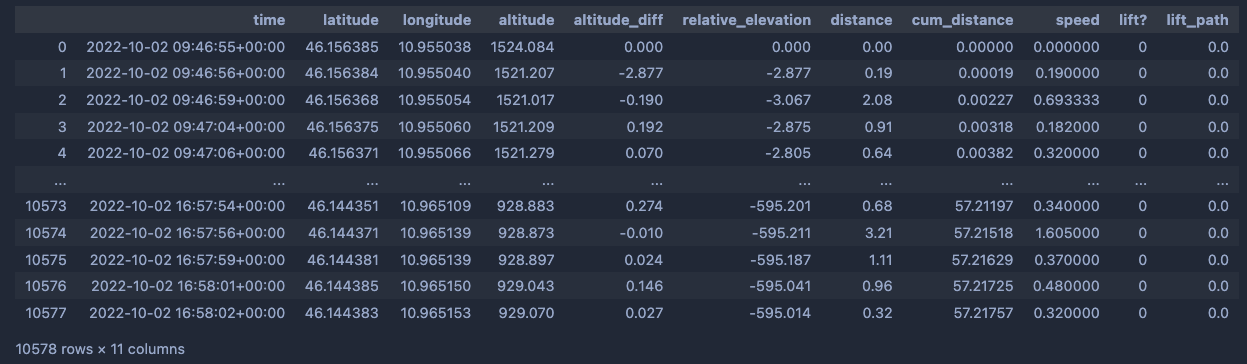
\includegraphics[width=\textwidth]{resources/df_loaded.png}
	\caption{The loaded DataFrame}
	\label{fig:df}
\end{figure}

In the next step the dependent and independent variables are defined.

\begin{lstlisting}[language=Python]
from sklearn.model_selection import train_test_split

# Select relevant features (columns)
features = ["distance", "speed", "altitude_diff"]

# Define the target column
target = "lift?"

# Split the data into features (X) and target (y)
X = data[features]
y = data[target]

# Split the data into training and testing sets
X_train, X_test, y_train, y_test = train_test_split(X, y, test_size=0.2, random_state=42)
\end{lstlisting}

By running the following command, the size of the independent variable X is determined:

\begin{lstlisting}[language=Python]
# Display the shape of the training and testing sets
print("x_train shape:", X_train.shape)
print("x_test shape:", X_test.shape)

# output:
	x_train shape: (8462, 3)
	x_test shape: (2116, 3)
\end{lstlisting}




\section{Approaches used}

As the project is classification \cite{osisanwo2017supervised}, the following approaches are used.

\subsection{Logistic Regression}
Logistic regression is a common statistical technique adapted for machine learning. It is suited for binary classification tasks where the target variable has two possible classes. Logistic regression models the probability of an observation belonging to each class. The logistic function ensures the probabilities are between 0 and 1 \cite{hosmer2013applied}.

Regression coefficients are learned during training to associate each feature with the log odds of the target. Important considerations when training logistic regressions include handling class imbalance and avoiding overfitting. Regularization methods like L1 and L2 can help prevent overfitting. Logistic regression is easy to implement, fast to train, and interpretable, but may not achieve best-in-class accuracy.


\begin{lstlisting}[language=Python]
	from sklearn import linear_model
	
	model_lr = linear_model.LogisticRegression(
	multi_class="multinomial", solver="lbfgs", max_iter=120, verbose=True)
	model_lr.fit(X_train, y_train)
	
\end{lstlisting}


\subsection{Random Forest}

Random forest is an ensemble method that trains multiple decision trees on subsets of data and features, combining their predictions through voting or averaging. By training on subsets, the decision trees exhibit greater diversity, reducing overfitting. Random forests achieve strong predictive accuracy by aggregating across many decision trees to smooth out individual errors \cite{breiman2001random}.

Tuning key hyperparameters like number of trees, maximum depth, and minimum samples per leaf can improve random forest performance. Feature importance scores can be calculated to understand impact on predictions. Random forests are accurate and robust to noise, but lose interpretability compared to simpler models. They can be prone to overfitting with noisy or complex data.

\subsection{Neural Networks}

Artificial neural networks are computing systems inspired by animal brains. They contain interconnected nodes called neurons arranged in layers. Input features are fed into input neurons, transformed through hidden layers of neurons via weighted connections, and output from output neurons. Neural nets learn by adjusting connection weights during training to minimize prediction error \cite{picton1994neural}.

Deep neural networks contain more hidden layers enabling modeling of complex nonlinear relationships in data. Key considerations include network topology and hyperparameter selection. Neural networks can model complex interactions between features that other models may miss. However, they require substantial data for training and are difficult to interpret compared to other techniques.

\section{Summary}

This section has provided an overview of key machine learning modeling concepts like features, target variables, and training data. Introductory explanations of three major algorithms - logistic regression, random forests, and neural networks - were also presented. These descriptions aim to establish essential foundational knowledge before diving into modeling details and experiments in subsequent chapters.


\section{model Section 1}
\label{sec:model:sec1}



\section{model Section 2}
\label{sec:model:sec2}


\section{model Section 3}
\label{sec:model:sec3}



\section{Conclusion}
\label{sec:model:conclusion}


         % INCLUDE: modeling
% !TEX root = ../my-thesis.tex
%
\chapter{Results}
\label{sec:results}



\section{Concepts Section 1}
\label{sec:concepts:sec1}



\section{Concepts Section 2 with a very very long title that illustrates how long section titles are handled in the footer}
\label{sec:concepts:sec2}



\section{Concepts Section 3}
\label{sec:concepts:sec3}



\section{Conclusion}
\label{sec:concepts:conclusion}


       % INCLUDE: results
% !TEX root = ../my-thesis.tex
%
\chapter{Conclusion}
\label{sec:conclusion}

\Blindtext[2][1]

\section{System Section 1}
\label{sec:conclusion:sec1}

\Blindtext[2][2]

\section{System Section 2}
\label{sec:conclusion:sec2}

\Blindtext[3][2]

\section{Future Work}
\label{sec:conclusion:future}

\Blindtext[2][2]
     % INCLUDE: conclusion

% --------------------------
% Back matter
% --------------------------
%
{%
\setstretch{1.1}
\renewcommand{\bibfont}{\normalfont\small}
\setlength{\biblabelsep}{0pt}
\setlength{\bibitemsep}{0.5\baselineskip plus 0.5\baselineskip}
\printbibliography[nottype=online]
\newrefcontext[labelprefix={@}]
\printbibliography[heading=subbibliography,title={Webpages},type=online]
}
\cleardoublepage

\listoffigures
\cleardoublepage

\listoftables
\cleardoublepage

\lstlistoflistings
\cleardoublepage

\appendix\cleardoublepage
% !TEX root = ../my-thesis.tex
%
\chapter{Example Appendix}
\label{sec:appendix}

\Blindtext[1][1]

\section{Appendix Section 1}
\label{sec:appendix:sec1}

\Blindtext[1][1]

\begin{table}[h]
	\begin{tabularx}{\textwidth}{X | X | X}
		%\hline
		Alpha		& Beta			& Gamma			\\ \hline
		0			& 1				& 2				\\ \hline
		3			& 4				& 5				\\ %\hline
	\end{tabularx}
	\label{tab:table1}
	\caption{This is a caption text.}
\end{table}

\section{Appendix Section 2}
\label{sec:appendix:sec2}

\Blindtext[1][1]

\begin{table}[h]
	\begin{tabularx}{\textwidth}{X | X | X}
		%\hline
		Alpha		& Beta			& Gamma			\\ \hline
		0			& 1				& 2				\\ \hline
		3			& 4				& 5				\\ %\hline
	\end{tabularx}
	\label{tab:table2}
	\caption{This is a caption text.}
\end{table}

\Blindtext[1][2]
       % INCLUDE: appendix

\cleardoublepage
% !TEX root = ../my-thesis.tex
%
\pagestyle{empty}
\hfill
\vfill
\pdfbookmark[0]{Colophon}{Colophon}
\section*{Colophon}

This thesis was typeset with \LaTeXe.
The design of the \textit{Clean Thesis} style is inspired by user guide documents from Apple Inc.

Download the \textit{Clean Thesis} style at \url{http://cleanthesis.der-ric.de/}.


\cleardoublepage
% !TEX root = ../my-thesis.tex
%
%************************************************
% Declaration
%************************************************
\pdfbookmark[0]{Declaration}{Declaration}
\addchap{Declaration}
\label{sec:declaration}
\thispagestyle{empty}

You can put your declaration here, to declare that you have completed your work solely and only with the help of the references you mentioned.

\bigskip

\noindent\textit{\thesisUniversityCity, \thesisDate}

\smallskip

\begin{flushright}
	\begin{minipage}{5cm}
		\rule{\textwidth}{1pt}
		\centering\thesisName
	\end{minipage}
\end{flushright}

%*****************************************
%*****************************************

\clearpage

\newpage
\mbox{}

% **************************************************
% End of Document CONTENT
% **************************************************
\end{document}
